\documentclass{article}
%%%%%%%%%%%%%%%%%%%%%%%%%%%%%%%%%%%%%%%%%
% Lachaise Assignment
% Structure Specification File
% Version 1.0 (26/6/2018)
%
% This template originates from:
% http://www.LaTeXTemplates.com
%
% Authors:
% Marion Lachaise & François Févotte
% Vel (vel@LaTeXTemplates.com)
%
% License:
% CC BY-NC-SA 3.0 (http://creativecommons.org/licenses/by-nc-sa/3.0/)
% 
%%%%%%%%%%%%%%%%%%%%%%%%%%%%%%%%%%%%%%%%%

%----------------------------------------------------------------------------------------
%	PACKAGES AND OTHER DOCUMENT CONFIGURATIONS
%----------------------------------------------------------------------------------------

%\usepackage{amsmath,amsfonts,stmaryrd,amssymb} % Math packages
\usepackage{amsmath,amsfonts,amssymb} % Math packages
\usepackage{enumerate} % Custom item numbers for enumerations

%\usepackage[ruled]{algorithm2e} % Algorithms

\usepackage[framemethod=tikz]{mdframed} % Allows defining custom boxed/framed environments

\usepackage{listings} % File listings, with syntax highlighting
\lstset{
	basicstyle=\ttfamily, % Typeset listings in monospace font
}

%----------------------------------------------------------------------------------------
%	DOCUMENT MARGINS
%----------------------------------------------------------------------------------------

\usepackage{geometry} % Required for adjusting page dimensions and margins

\geometry{
	paper=a4paper, % Paper size, change to letterpaper for US letter size
	top=2.5cm, % Top margin
	bottom=2.5cm, % Bottom margin
	left=2.5cm, % Left margin
	right=2.5cm, % Right margin
	headheight=14pt, % Header height
	footskip=1.5cm, % Space from the bottom margin to the baseline of the footer
	headsep=1.2cm, % Space from the top margin to the baseline of the header
	%showframe, % Uncomment to show how the type block is set on the page
}

%----------------------------------------------------------------------------------------
%	FONTS
%----------------------------------------------------------------------------------------

\usepackage[utf8]{inputenc} % Required for inputting international characters
\usepackage[T1]{fontenc} % Output font encoding for international characters

%\usepackage{XCharter} % Use the XCharter fonts

%----------------------------------------------------------------------------------------
%	COMMAND LINE ENVIRONMENT
%----------------------------------------------------------------------------------------

% Usage:
% \begin{commandline}
%	\begin{verbatim}
%		$ ls
%		
%		Applications	Desktop	...
%	\end{verbatim}
% \end{commandline}

\mdfdefinestyle{commandline}{
	leftmargin=10pt,
	rightmargin=10pt,
	innerleftmargin=15pt,
	middlelinecolor=black!50!white,
	middlelinewidth=2pt,
	frametitlerule=false,
	backgroundcolor=black!5!white,
	frametitle={Command Line},
	frametitlefont={\normalfont\sffamily\color{white}\hspace{-1em}},
	frametitlebackgroundcolor=black!50!white,
	nobreak,
}

% Define a custom environment for command-line snapshots
\newenvironment{commandline}{
	\medskip
	\begin{mdframed}[style=commandline]
}{
	\end{mdframed}
	\medskip
}

%----------------------------------------------------------------------------------------
%	FILE CONTENTS ENVIRONMENT
%----------------------------------------------------------------------------------------

% Usage:
% \begin{file}[optional filename, defaults to "File"]
%	File contents, for example, with a listings environment
% \end{file}

\mdfdefinestyle{file}{
	innertopmargin=1.6\baselineskip,
	innerbottommargin=0.8\baselineskip,
	topline=false, bottomline=false,
	leftline=false, rightline=false,
	leftmargin=2cm,
	rightmargin=2cm,
	singleextra={%
		\draw[fill=black!10!white](P)++(0,-1.2em)rectangle(P-|O);
		\node[anchor=north west]
		at(P-|O){\ttfamily\mdfilename};
		%
		\def\l{3em}
		\draw(O-|P)++(-\l,0)--++(\l,\l)--(P)--(P-|O)--(O)--cycle;
		\draw(O-|P)++(-\l,0)--++(0,\l)--++(\l,0);
	},
	nobreak,
}

% Define a custom environment for file contents
\newenvironment{file}[1][File]{ % Set the default filename to "File"
	\medskip
	\newcommand{\mdfilename}{#1}
	\begin{mdframed}[style=file]
}{
	\end{mdframed}
	\medskip
}

%----------------------------------------------------------------------------------------
%	NUMBERED QUESTIONS ENVIRONMENT
%----------------------------------------------------------------------------------------

% Usage:
% \begin{question}[optional title]
%	Question contents
% \end{question}

\mdfdefinestyle{question}{
	innertopmargin=1.2\baselineskip,
	innerbottommargin=0.8\baselineskip,
	roundcorner=5pt,
	nobreak,
	singleextra={%
		\draw(P-|O)node[xshift=1em,anchor=west,fill=white,draw,rounded corners=5pt]{%
		Question \theQuestion\questionTitle};
	},
}

\newcounter{Question} % Stores the current question number that gets iterated with each new question

% Define a custom environment for numbered questions
\newenvironment{question}[1][\unskip]{
	\bigskip
	\stepcounter{Question}
	\newcommand{\questionTitle}{~#1}
	\begin{mdframed}[style=question]
}{
	\end{mdframed}
	\medskip
}

%----------------------------------------------------------------------------------------
%	WARNING TEXT ENVIRONMENT
%----------------------------------------------------------------------------------------

% Usage:
% \begin{warn}[optional title, defaults to "Warning:"]
%	Contents
% \end{warn}

\mdfdefinestyle{warning}{
	topline=false, bottomline=false,
	leftline=false, rightline=false,
	nobreak,
	singleextra={%
		\draw(P-|O)++(-0.5em,0)node(tmp1){};
		\draw(P-|O)++(0.5em,0)node(tmp2){};
		\fill[black,rotate around={45:(P-|O)}](tmp1)rectangle(tmp2);
		\node at(P-|O){\color{white}\scriptsize\bf !};
		\draw[very thick](P-|O)++(0,-1em)--(O);%--(O-|P);
	}
}

% Define a custom environment for warning text
\newenvironment{warn}[1][Warning:]{ % Set the default warning to "Warning:"
	\medskip
	\begin{mdframed}[style=warning]
		\noindent{\textbf{#1}}
}{
	\end{mdframed}
}

%----------------------------------------------------------------------------------------
%	INFORMATION ENVIRONMENT
%----------------------------------------------------------------------------------------

% Usage:
% \begin{info}[optional title, defaults to "Info:"]
% 	contents
% 	\end{info}

\mdfdefinestyle{info}{%
	topline=false, bottomline=false,
	leftline=false, rightline=false,
	nobreak,
	singleextra={%
		\fill[black](P-|O)circle[radius=0.4em];
		\node at(P-|O){\color{white}\scriptsize\bf i};
		\draw[very thick](P-|O)++(0,-0.8em)--(O);%--(O-|P);
	}
}

% Define a custom environment for information
\newenvironment{info}[1][Info:]{ % Set the default title to "Info:"
	\medskip
	\begin{mdframed}[style=info]
		\noindent{\textbf{#1}}
}{
	\end{mdframed}
}

\usepackage[czech]{babel}

\usepackage{graphicx} % Required for including images
\graphicspath{{./}}   % Location of the graphics files
\usepackage[font=small,labelfont=bf]{caption} % Required for specifying captions to tables and figures
\usepackage{booktabs}
\newcommand{\Celsius}{$^\circ$C}

%-------------------------------------------------------------------------------
%	ASSIGNMENT INFORMATION
%-------------------------------------------------------------------------------

\title{Cvičení ze statistických metod č. 1} % Title of the assignment

\author{Michaela Štefková, 458194} % jméno, učo

\date{\today} % date

%-------------------------------------------------------------------------------

\begin{document}
	
	\maketitle % Print the title
	
	%----------------------------------------------------------------------------------------
	%	ZADÁNÍ
	%----------------------------------------------------------------------------------------
	\part*{Úkol č. 3}
	\section*{Zadání} % Unnumbered section
	
	V programu Statistika vypočtěte z přiložených dat teplota.xls ve studijních materiálech průměr, směrodatnou odchylku, minimum a maximum pro každý měsíc v letech 1961--2000. Dále vypočtěte maximální teplotu pro každý rok.
	
	%----------------------------------------------------------------------------------------
	%	POSTUP
	%----------------------------------------------------------------------------------------
	
	\section*{Postup} % Unnumbered section
	
	Ze studijních materiálů předmětu stáhneme soubor teplota.xls. Načteme soubor teplota.xls do programu Statistica. Přidáme proměnnou, kterou nazveme Rok. Vypočítáme průměrnou roční teplotu vzduchu. Vypočítáme průměr, směrodatnou odchylku, minimum a maximum pro každý měsíc. 
	Pomocí „statistik bloku dat“ vypočítáme průměr pro všechny měsíce a pro každý rok vypočítáme maximální teplotu.
	
	\section*{Vypracování}
	
  \begin{table}[ht]\centering \renewcommand{\arraystretch}{1.4}
 	\caption{Popisné statistiky ve všech měsících v období 1961--2000}
 	\begin{tabular}{@{}crrrr@{}}\toprule
 		       & \multicolumn{4}{c}{Popisné statistiky (teplota [\Celsius])} \\ 
 		       & Průměr   & Minimum  & Maximum  & Sm. odchylka \\ \midrule
 		  I    & -2,11500 & -7,90000 & 3,30000  & 2,695157     \\ %\hline
 		  II   & -0,27500 & -6,70000 & 5,00000  & 2,847198     \\ %\hline
 		  III  & 3,67000  & -1,40000 & 7,50000  & 2,345776     \\ %\hline
 		  IV   & 8,80250  & 5,90000  & 12,70000 & 1,482113     \\ %\hline
 		  V    & 13,61500 & 9,80000  & 16,10000 & 1,442141     \\ %\hline
 		  VI   & 16,80750 & 14,50000 & 18,90000 & 1,150783     \\ %\hline
 		  VII  & 18,70500 & 16,30000 & 22,70000 & 1,584694     \\ %\hline
 		  VIII & 18,39750 & 15,80000 & 23,20000 & 1,438569     \\ %\hline
 		  IX   & 14,29500 & 10,70000 & 17,30000 & 1,471603     \\ %\hline
 		  X    & 8,96750  & 5,60000  & 12,60000 & 1,412833     \\ %\hline
 		  XI   & 3,25000  & 0,00000  & 7,00000  & 1,747085     \\ %\hline
 		  XII  & -0,68250 & -5,60000 & 3,50000  & 2,084483     \\ \bottomrule
 	\end{tabular}
 \end{table}

 
 \begin{table}[p]\centering \renewcommand{\arraystretch}{1.2}
	\caption{Maximální teplota pro každý rok v období 1961--2000}
	\begin{tabular}{cc}\toprule
		 Rok & \multicolumn{1}{c}{Maximální teplota [\Celsius]} \\ \midrule
		 1961   &  18,1 \\ 
		 1962   &  19,1 \\ 
		 1963   &  20,4 \\ 
		 1964   &  19,7 \\ 
		 1965   &  17,3 \\ 
		 1966   &  17,6 \\ 
		 1967   &  20,2 \\ 
		 1968   &  18,4 \\ 
		 1969   &  19   \\  
		 1970   &  18,4 \\ 
		 1971   &  20,5 \\ 
		 1972   &  19,2 \\ 
		 1973   &  19,6 \\ 
		 1974   &  19,8 \\ 
		 1975   &  19,1 \\ 
		 1976   &  20   \\  
		 1977   &  18,2 \\ 
		 1978   &  16,7 \\ 
		 1979   &  18,9 \\ 
		 1980   &  17,8 \\ 
		 1981   &  18,6 \\ 
		 1982   &  19,4 \\ 
		 1983   &  22,4 \\ 
		 1984   &  17,6 \\ 
		 1985   &  18,6 \\ 
		 1986   &  17,9 \\ 
		 1987   &  18,9 \\ 
		 1988   &  19,5 \\ 
		 1989   &  19,1 \\ 
		 1990   &  19,9 \\ 
		 1991   &  20,6 \\ 
		 1992   &  23,2 \\ 
		 1993   &  18,8 \\ 
		 1994   &  22,7 \\ 
		 1995   &  22   \\  
		 1996   &  17,6 \\ 
		 1997   &  19,6 \\ 
		 1998   &  19,6 \\ 
		 1999   &  19,6 \\ 
		 2000   &  20,1 \\ 
		\bottomrule
	\end{tabular} 
	\label{fig:tab1}
\end{table}
	
\newpage
	\maketitle % Print the title
	 	
	 %----------------------------------------------------------------------------------------
	 %	ZADÁNÍ
	 %----------------------------------------------------------------------------------------
	 	
	 \part*{Úkol č. 4}
	 \section*{Zadání} % Unnumbered section
	 	
	 	Vytvořte z dat teplota.xls ve studijních materiálech spojnicový graf pro leden 1961--2000, zobrazující lineární trend. Vypočtěte průměrné hodnoty a vytvořte novou proměnnou dif leden a do ní vypočítejte diferenci teploty od průměru. 
	 	
 	 	
	 	%----------------------------------------------------------------------------------------
	 	%	POSTUP
	 	%----------------------------------------------------------------------------------------
	 		
	 	\section*{Postup} % Unnumbered section
	 	
	 			
		Z dat ve studijních materiálech si vytvoříme spojnicový graf pro měsíc leden za období 1961--2000, upravíme  názvy os a spojnicovou linii a do grafu přidáme lineární trend. Pro měsíc leden vypočteme diference teploty od průměru za období 1961--2000. Pro tyto diference vytvoříme sloupcový graf.
		
		\section*{Vypracování}

	\begin{figure}[h]
	\centering
	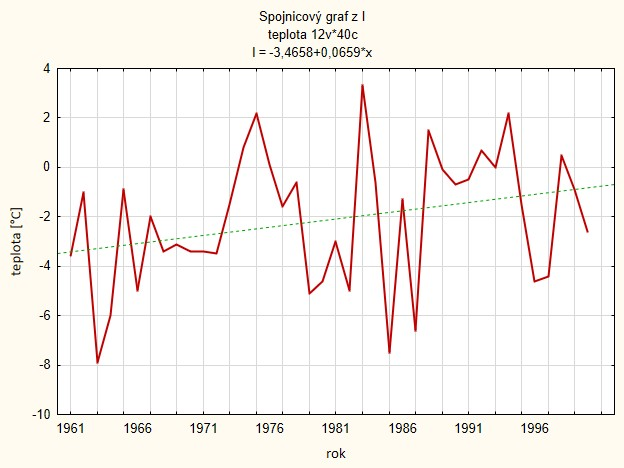
\includegraphics[width=0.9\linewidth]{Stats1.jpg}
	\caption{Vývoj teploty v měsíci lednu pro období 1961--2000, zobrazující literární trend}
	\label{fig:GrafinStats1}
	\end{figure}

\begin{figure}
\centering
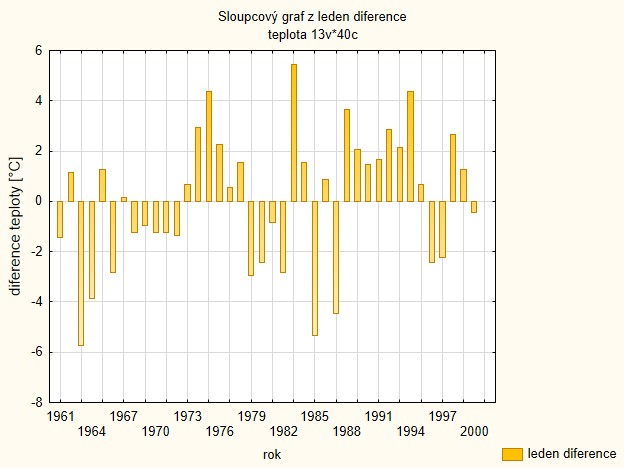
\includegraphics[width=0.9\linewidth]{GrafinPS1}
\caption{Diference teploty od průměrné teploty v měsíci lednu v letech 1961--2000}
\label{fig:GrafinPS1}
\end{figure}

\end{document}
